\documentclass[12pt]{article}

\usepackage{upgreek}

\usepackage{amsmath}

\usepackage{graphicx}

\usepackage{dsfont}

\usepackage{hyperref}

\usepackage[utf8]{inputenc}

\usepackage{graphicx}
\graphicspath{ {imgs/} }

\usepackage{mathtools}

\usepackage{textcomp}

\usepackage[english]{babel}

\usepackage{tikz}

\usepackage{tcolorbox}

\usepackage{amsthm,amssymb}

\setlength{\parindent}{0cm}

\renewcommand\qedsymbol{$\blacksquare$}

\usepackage{fancyhdr}
 
\pagestyle{fancy}
\fancyhf{}
\fancyhead[LE,RO]{Introduction to Databases -- Fall 2017}
\fancyhead[RE,LO]{Joshua Concon}
\fancyfoot[CE,CO]{\leftmark}
\fancyfoot[LE,RO]{\thepage}


\begin{document}

\title{CSCC43: Introduction to Databases\\ Lecture Notes}
\date{University of Toronto Scarborough -- Fall 2017}
\author{Joshua Concon}
\maketitle
Pre-reqs are CSCB63 and STAB52.
Instructor is Dr. Marzieh Ahmadzadeh. Check RateMyProf. If you find any problems in these notes, feel free to contact me at conconjoshua@gmail.com. I own nothing, all copyrighted works belong to their respective owners (University of Toronto and Pearson Education).

\tableofcontents

\pagebreak

\section{Thursday, September 7, 2017}

\subsection{Definitions}

\paragraph{Data} Objects or events that could be recorded on a computer media. This includes stuff like an email, an address, a student identification number, etc.\\

However, there are two types of Data, Unstructured and Structured.

\paragraph{Structured Data} They are mostly stored in a tabular format, have types including: date, character, numeric, alphanumeric.

\paragraph{Unstructured Data} Data that must be analyzed to extract information from, does not already show information. Includes multimedia, maps, documents, pictures, voices.

\paragraph{Database} An organized collection of logically related data that can be of any size or complexity. Example:
\begin{itemize}
	\item{Student ID, name, GPA, courses taken}
	\item{Patient name, doctor's ID, ward, date of admission}
	\item{Personnel ID, base salary, bonus, hours of work}
\end{itemize}

\underline{Another Example:}

\begin{center}
 \begin{tabular}{||c c c||} 
 \hline
 ID & Course & Mark \\ [0.5ex] 
 \hline\hline
 100 & CSCC43 & A \\ 
 \hline
 100 & CSCC44 & B \\
 \hline
 100 & CSCC52 & A+  \\
 \hline
 200 & CSCC43 & A+\\
 \hline
 200 & CSCC62 & B\\ [1ex] 
 \hline
\end{tabular}
\end{center}

\paragraph{Database Management System (DBMS)} A software that sits between users and databases, responsibilities include:
\begin{itemize}
	\item{Allowing users to create, update, sort or retrieve data}
	\item{Enforcing the integrity of data (consistency, etc.)}
	\item{Improving performance when dealing with huge data or many queries}
	\item{Assuring the durability of the data}
	\item{Allowing data to be shared among different programs}
	\item{managing concurrent access by multiple users/processes}
\end{itemize}

\paragraph{Information} Information is data that has been process in order to increase user knowledge, could be data provided in a way that can be analyzed easily (i.e. has labels, maybe graphs showing relationships, etc.)

\paragraph{Metadata} "Data about data". Data that describes the properties of end-user data and it's context, it helps the database designer understand what kind of data exists and what it means. Examples include name, type, length, allowable values, ownership (stewardship), source...
\\
\underline{Example:}\\
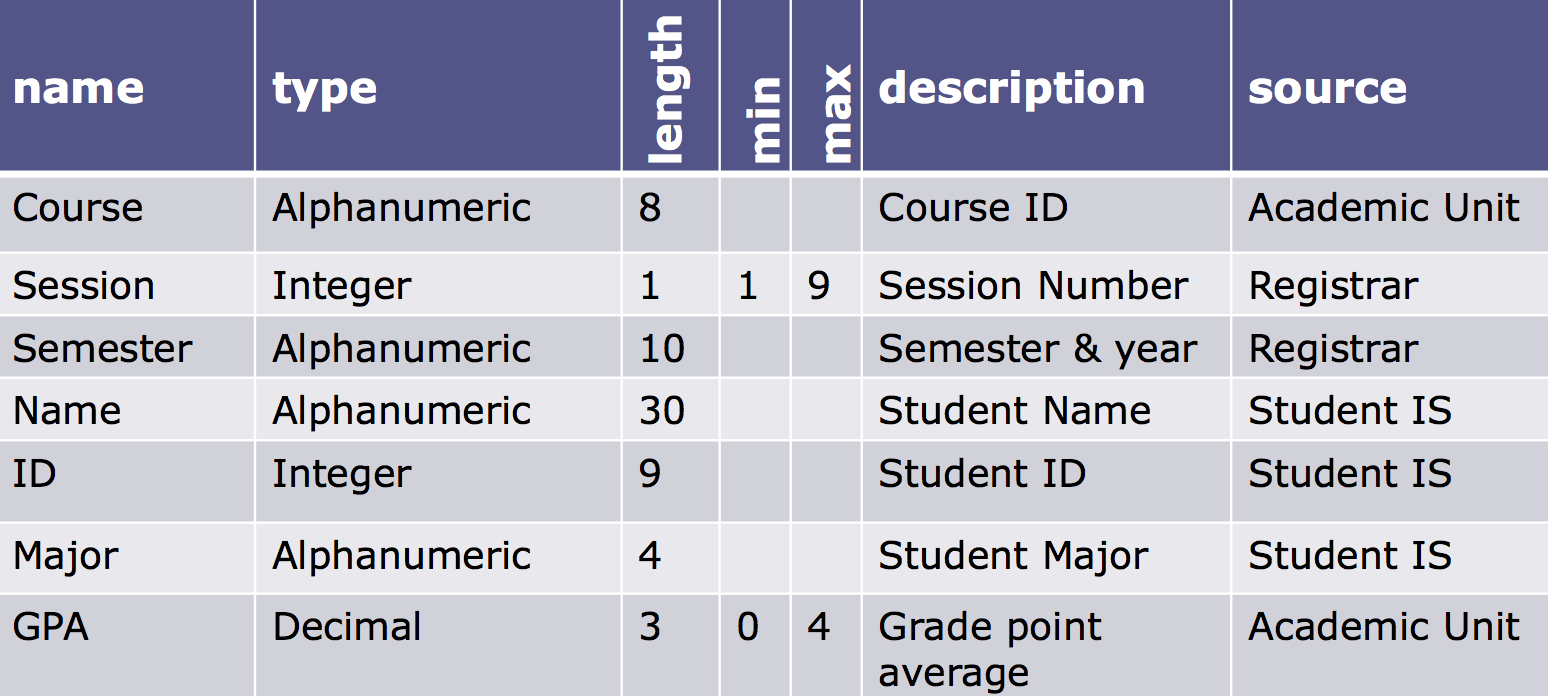
\includegraphics[scale=0.5]{lec1-1}

\subsection{How do we store data?}

There are two ways we can store data, either the Traditional file system or the database approach.

\subsubsection{Traditional File System}

The Traditional File System includes files that are also collections of related data, was used prior to the invention of databases, but has its own disadvantages.\\
\\
\underline{Example of a file system:}\\
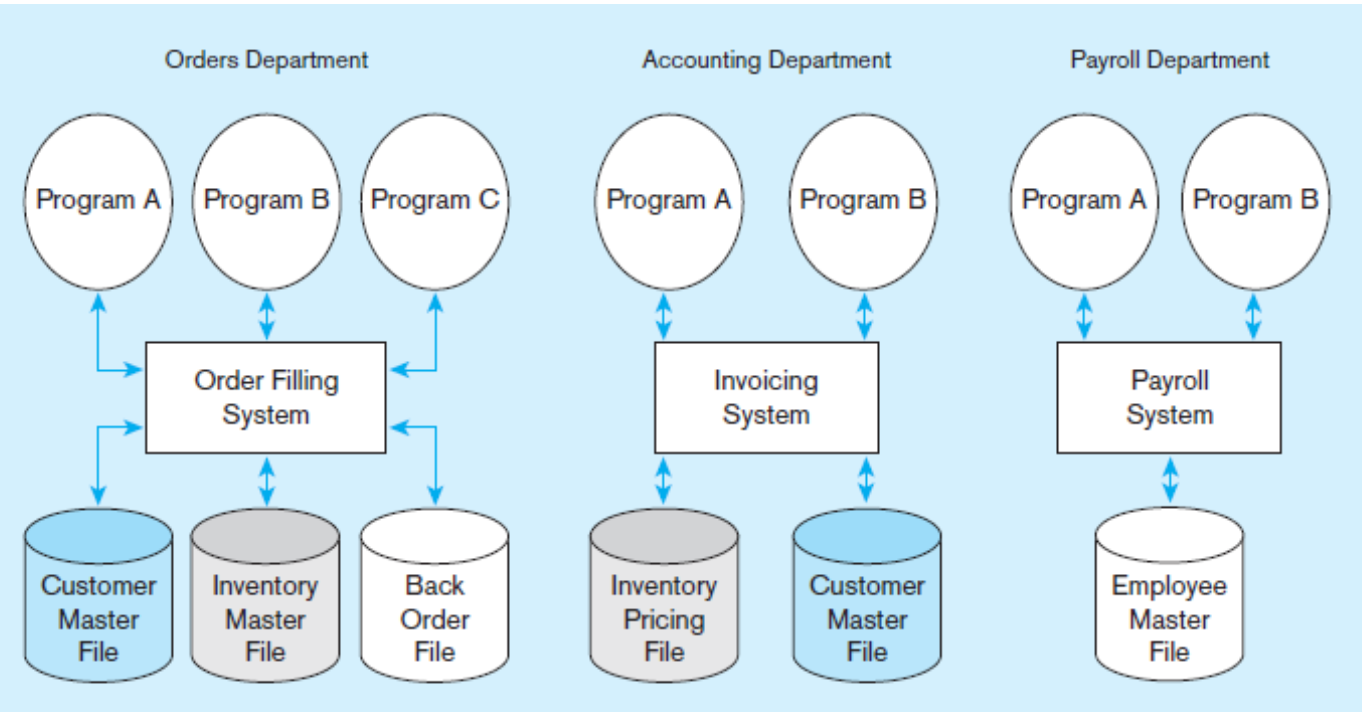
\includegraphics[scale=0.5]{lec1-2}\\

\underline{Disadvantages:}
\paragraph{Program-Data Dependence} If the data is changes, all programs that used the data should be altered to. To use an example from the previous image, if the length of data such as customer name is changed, order filling system programs and invoice system programs are both affected. Using the database approach, this is managed by a Database Management System and no change in order filling or account programs are required, only on the file itself.

\paragraph{Duplication of Data} As seen from the last image, the order filling system and the invoice system both have a customer master file. This is a waste of space as it is essentially two sets of the same data, and reliable metadata is difficult to establish since it may be inconsistent. Changes to one copy must also be applied to the other, so this may compromises the files' data integrity.

\paragraph{Limited Data Sharing} Since each application has its own data, data sharing between applications is not easy, a system does not have access to another system's data. With the database approach, data sharing is doable.

\paragraph{Length Development Times} Each new application should be started from scratch by designing a new file format and description, however, in the database approach, you only need to design your database once, and can easily access the data you need.

\paragraph{Excessive Program Maintenance} All preceding factors creates heavy program maintenance, so to avoid these disadvantages, the database approach is preferred. Note that if a database is not properly designed, mentioned disadvantages may not disappear.

\subsubsection{Database Approach}

The database approach creates a repository of shared data, data is managed by a controlling agent (Database Management System), and all data is stored in a standardized convenient form.\\
\\
\underline{Visualization Example:}\\
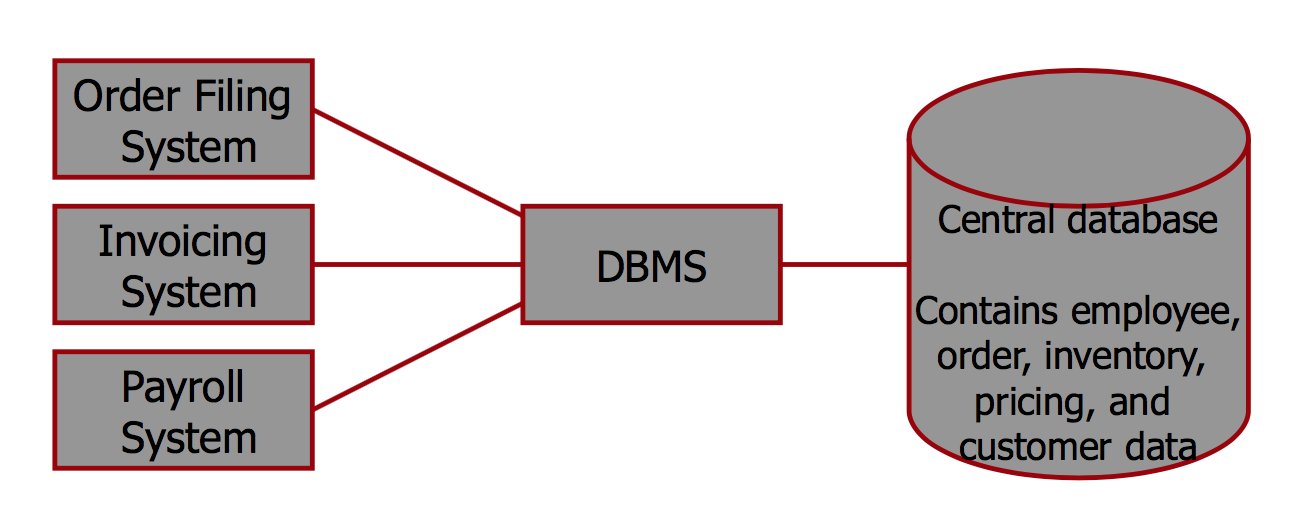
\includegraphics[scale=0.5]{lec1-3}\\

Every Database uses a data model, and this data model is a notation for describing data that specifies the structure of the data, the constrains on the content of the data, and the operations on the data.\\
\\
Some examples of data models include a relational data model, a semistructured data model, unstructured data, and an Object-oriented model.

\subsection{Relational Data Model}

The main concept of the relational data model is a relation, which is based off the concept of relations in math. A relation in a database is like a table consisting of rows and columns.\\
\\
\underline{Example:}\\
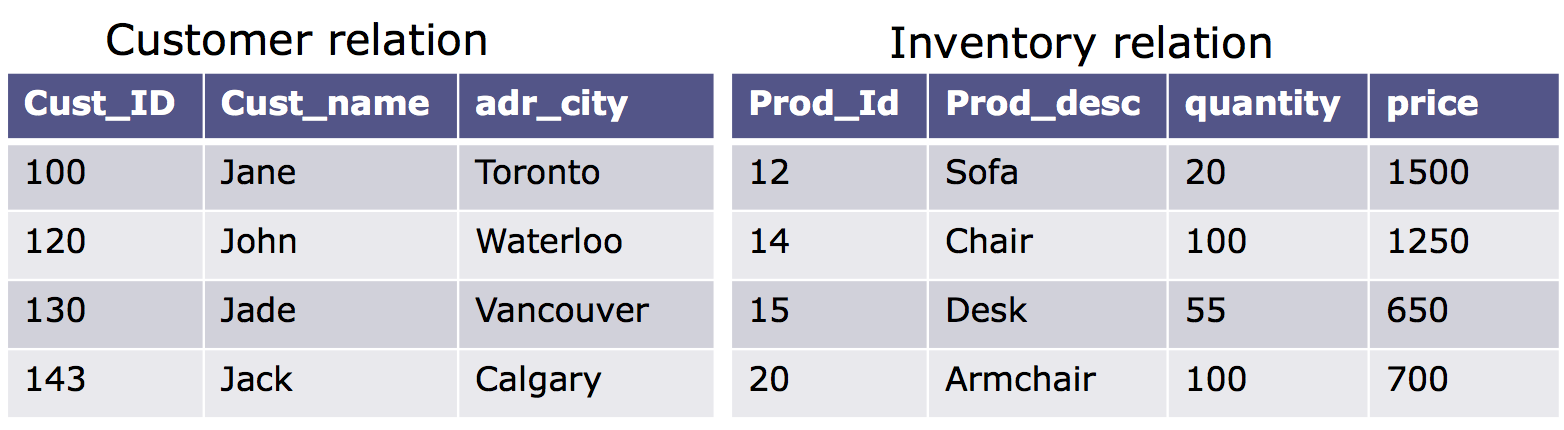
\includegraphics[scale=0.5]{lec1-4}\\

\subsubsection{Advantages}

\paragraph{Program-data independence} Metadata is stored in a central location called a repository, and data could be changed independent of what program uses it.

\paragraph{Planned data redundancy} Data is only duplicated when we want it to be duplicated, so we can control redundancy.

\paragraph{Improved data consistency} Which is implied since data redundancy is eliminated.

\paragraph{Increased productivity of application development} Since the application does not deal with the data management, since it is taken care of by the Database Management System, so time and cost of development is saved.

\paragraph{Enforcement of standards} Standards are enforced by the uniform procedures for accessing and updating data.

\paragraph{Improved data quality} By defining constraints that the data must follow.

\paragraph{Improved data accessibility and responsiveness} Can be done by using a query system to access data.

\paragraph{Reduced program maintenance} Because of data-program independence, changing the data does not affect any program.

\paragraph{Improved data sharing} By creating a user view and since all applications share the same data already, data sharing is doable.

\subsubsection{Cost and Risk}

\paragraph{New specialized personnel} Companies need to hire new people for database design and database administration services.

\paragraph{Installation and Management of Cost and Complexity} Implementation of the database and scaling it will be a new concern for companies

\paragraph{Conversion Costs} Costs for converting legacy system to a modern database

\paragraph{Need for backup and recovery} New costs and concerns for backing up the database and new services companies must worry about for recovery.

\paragraph{Organizational Conflict} On data definition, data format and right to update data.

\subsection{Database Development Process}

\paragraph{Model the rule of the organization} Such as, "each student at UofT can take up to 5 courses in one semester"

\paragraph{Explore a relation between various entities} Such as, "A course might be taken by many students", "A student must take at least one course", etc.

\paragraph{Create your relation} Creating the tables with relations between the entities and data associated with each object

\paragraph{Normalize your relation} We will learn what this is later in the course

\paragraph{Implementation} Actual Implementation of the database

\newpage

\section{Thursday, September 14, 2017}

\subsection{Relational Data Model}

A relational data model has 3 components, one of which is an \textbf{Entity}, which contains the Entity itself: which is a concept that we maintain data about, an \textbf{Entity Type}: which corresponds to a table and what the information in the table refers to, and an \textbf{Entity Instance}, which is an instance of an entity, such as (100, Jane, 3.5), which refers to a student named Jane with a Student ID of 100 and a cGPA of 3.5.\\

The notation for the entities is as follows (It's mostly just a rectangle tbh):\\
\\
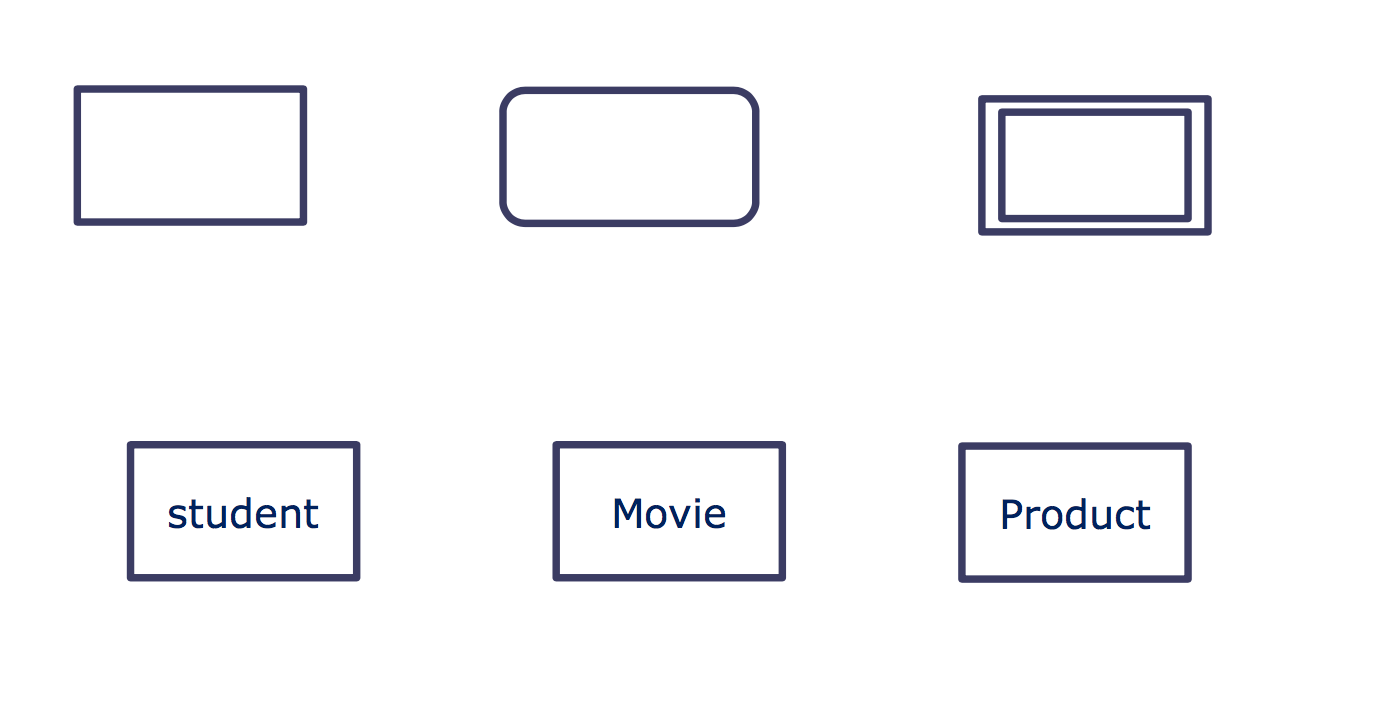
\includegraphics[scale=0.5]{lec2-1}


Another one of the 3 components is a \textbf{Relationship}, which contains a \textbf{Relationship Instance}: which is an association between entity instances itself, such as a Student named Jane taking 3 courses (which is a 1:M relationship as 1 student can take many courses) and a \textbf{Relationship Type}: which was the type of relationship, such as (1:M) as described in the previous example.\\
\\
The notation for relationship types is as follows:\\
\\
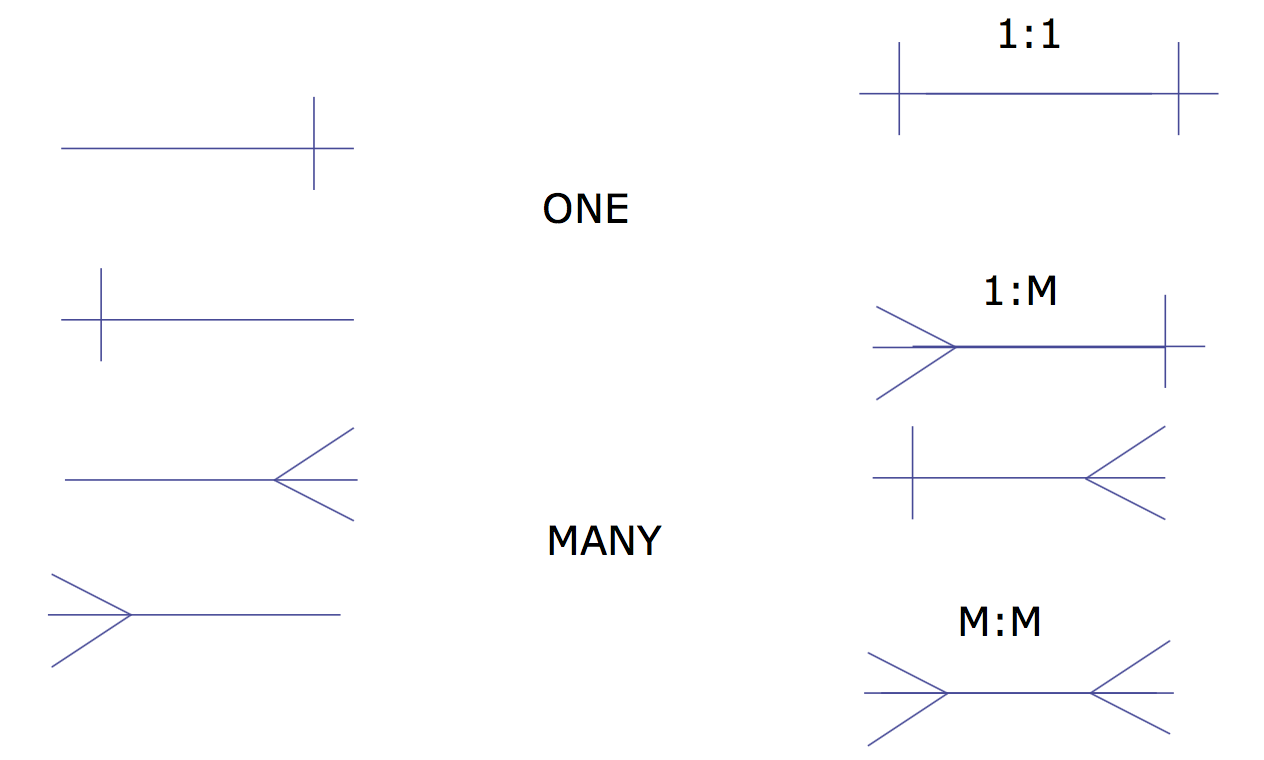
\includegraphics[scale=0.5]{lec2-2}

The last of the 3 components are \textbf{attributes}, which are properties or characteristics of an entity, which often corresponds to a field in a table. For example, for a student entity, an example attribute for this student entity would be "cgpa" or "student ID".

\subsection{Database Analysis}

Before the database can be created, you must first gather user requirements for the data, what exactly we need this data to do and what kind of constraints we need. We'll need to know the entities we would have to make for the database and what relationships these entities have with each other.\\
\\
Afterwards, we must develop a data model, more specifically, an Entity Relationship (ER) model.

\subsection{Business Rules}

Business Rules are statements that define or constrain some aspect of the business. For Example: "at UofT, a student must take at least one course in each semester." These statements are usually derived from policies, procedures, events, and functions, for example: "at UofT, a student should have passed the prerequisites to be able to take a course." These constraints and definitions must also be familiar to the end users and must be automatically enforced by the Database Management Software.\\
\\
We gather these business rules by speaking to people involved in the business that this database is being created for and by investigating business documents.

\subsubsection{Cardinality Constraints}

\textbf{Cardinality Constraints} are rules that specifies the number of instances of one entity that can be associated with each instance of another entity. Examples include:
\begin{itemize}
	\item{"Each student at UofT can take \underline{at most 5} courses each semester"}
	\item{"Each person can have \underline{at most 1} family doctor"}
	\item{"A movie can be screened \underline{at most 6} times a day"}
\end{itemize}

\textbf{Minimum Cardinality} is the minimum number of instances of one entity that can be related to the other instance.\\
\\
\textbf{Maximum Cardinality} is the maximum number of instances of one entity that may be related to each instance of another entity.\\
\\
The notation for these cardinality constraints are as such:\\
\\
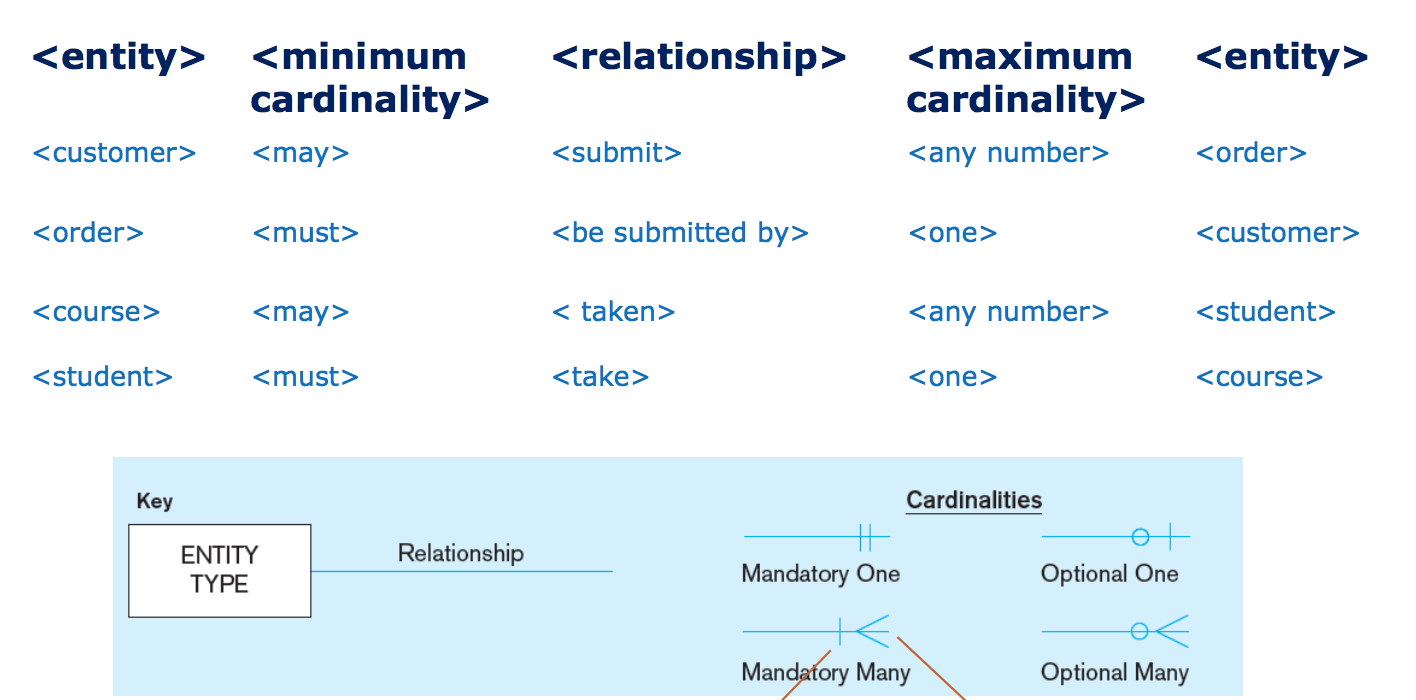
\includegraphics[scale=0.5]{lec2-3}

\subsection{Entity Relationship (ER) Model}

After business rules have been collected, from these rules, relationships between entities can be modelled, and for this, we will use the Entity Relationship Model. This model is a logical representation of the data for an organization, the entities are to represent the data, and the relationships are to show the associations between entities.

\subsubsection{Entity}

An entity is the building block of the Entity Relationship Model, such examples include:
\begin{itemize}
	\item{Person: \textit{employee, student, patient}}
	\item{Place: \textit{store, warehouse, state, drugstore}}
	\item{Object: \textit{machine, building, automobile}}
\end{itemize}

An entity is supposed to have a noun name and is meant to be general.\\
\\
Each entity usually consists of several \textbf{attributes.}\\
\\
An entity should be an object that will have many instances in the database, and object that will be composed of multiple attributes, and/or an object that we are trying to model. However, it should also not be a user of the database system or an output of the database system.

\subsubsection{The Weak shall fear the Strong}

There are two different types of Entities, \textbf{Strong} and \textbf{Weak} entities.\\
\\
\underline{Strong entities} exist independently of other types of entities and have their own unique identifier (e.g students, employee, course, surgeon, independent black woman who need no man).\\
\\
\underline{Weak entities} depend on a strong entity, which may or may not be their identifying owner, and cannot exist on it's own. They also do not have a unique identifier, only a partial identifier, and the entity box and partial identifier have double lines.\\
\\
The following is an example of a weak entity:\\
\\
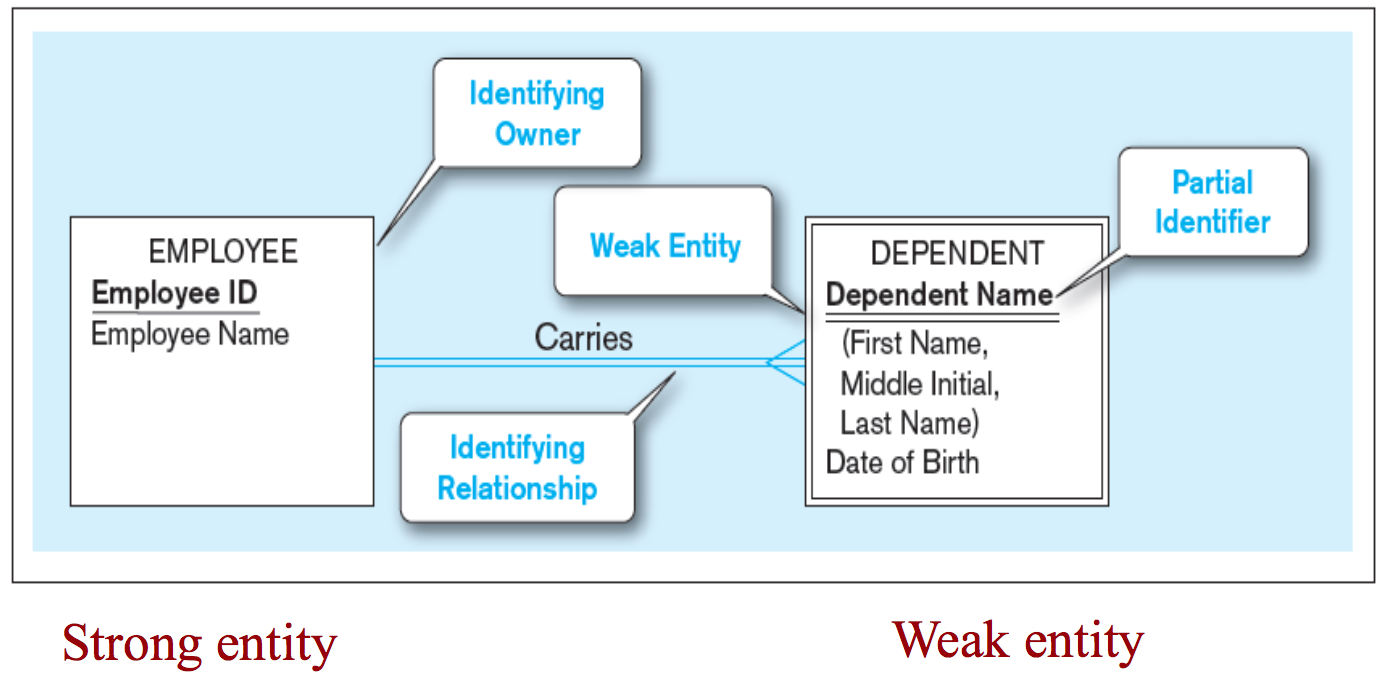
\includegraphics[scale=0.5]{lec2-4}

\subsubsection{Attributes}

Each entity type has a set of \textbf{attributes} associated with it, and by default, the name of an attribute starts with a capital.\\s
\\
An attribute has different types, including: required, optional, simple, composite, single values, multivalued, stored, derived, and identifier.
\paragraph{Required Attributes} Required Attributes should have a value. Must be boldfaced or represented by a special character in E-R Diagrams.

\paragraph{Optional Attributes} Optional Attributes can be null. May be represented by an 'o' in E-R Diagrams.

\paragraph{Composite Attributes} An attribute that has meaningful component parts. For example: an address can be broken down to city, street, etc. It is up to the user as how to define these attributes. If you might use only part of an attribute, you might want to separate it as its own attribute.

\paragraph{Simple Attributes} An attribute that cannot be broken down into smaller components, such as a StudentID.

\paragraph{Multivalued Attributes} An attribute that can have more that one value. For example, skill can be 'programmer', 'analyst', etc. This type of attribute is represented with curly braces {} in ER diagrams.

\paragraph{Single Valued Attributes} An attribute that can only have one value, such as an attribute that can only be a boolean (True or False).

\paragraph{Derived Attributes} An attribute that is derived from other stored attributes. For example, years employed can be derived from today's date minus date employed. This type of attribute is represented with square brackets [] in ER diagrams.

\paragraph{Stored Attributes} An attribute that is not derived from other stored attributes, and is just stored.

\paragraph{Identifier Attributes} An attribute whose value distinguishes instances of an entity type, so no two instances are referred to by one identifier, such as an EmployeeID for example.

\paragraph{Composite Identifier} An identifier that consists of a composite attribute.

For naming these attributes, it should be a unique singular noun or noun phrase such as 'Customer ID' or 'Product Minimum Price'. The name should also follow a standard for uniqueness, such as [Entity type name { [ Qualifier ] }] Class, where the Qualifier is a phrase to constrain the class, and the Class is the properties of the entities. An example of an attribute under this template is 'Customer hourly wage'. Similar attributes of different entity types should use the same qualifiers and classes, such as 'Faculty Residence City' and 'Student Residence City'.

\subsubsection{Criteria for Identifiers}

Identifiers must be values that will never be null and will not change in value. It is ideal to substitute new, simple keys for long, composite keys if possible.

\subsubsection{Modelling Relationships}

A relationship in E-R diagrams are modelled by verbs and is represented by a line labelled with the name of the relationship.

\paragraph{Degree of Relationships} The degree of a relationship is the number of entity types  that participate in it, so for example, a \textbf{Unary} relationship would refer to one entity related to another of the same type, a \textbf{Binary} relationship would refer to two different entities, a \textbf{Ternary} relationship would refer to three different entity types.

\newpage

\section{Thursday, September 21, 2017}

\subsection{Associative Entity}

When you have a many to many relationship, and that relationship requires to have attributes assigned to it, you can create an associative entity.\\
\\
\underline{Example:}\\
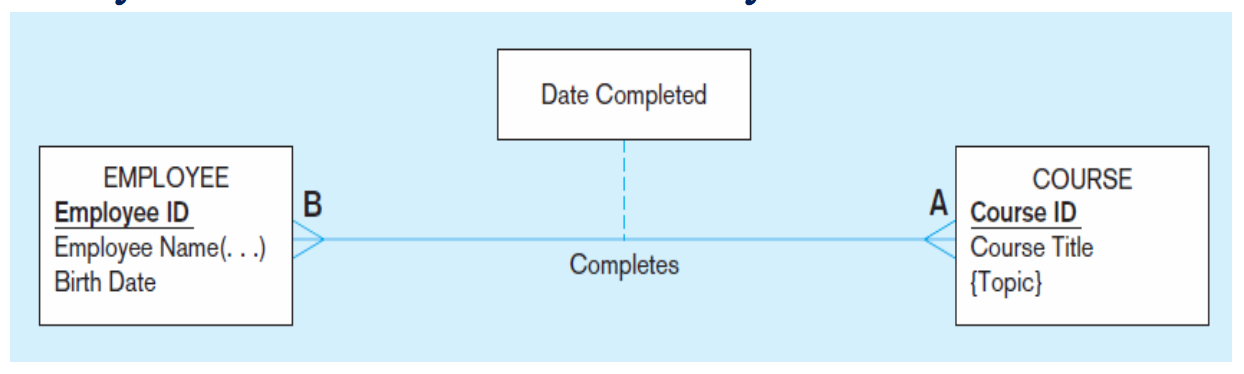
\includegraphics[scale=0.5]{lec3-1}

To denote an associative entity, you use a rounded box for the attributes, you define an identifier, and for a Many to Many relationship between entities $A$ and $B$, define the associative entity as $C$ and relate the entities as such $A:C$, as one to many and $B:C$ as one to many as well.\\
\\
\begin{tcolorbox}
	Note that Many to Many relationships cannot be implemented using a relational database.
\end{tcolorbox}

\subsection{Multiple Relationships}

It is possible that one entity can participate in more than one relationship. The relationship could be in any degree or cardinality (Mandatory or optional, any combination of 1 or many to 1 or many).\\
\\
\underline{Example:}\\
In $X$ Company, Sue manages 2 departments (finances and sale) in which 10 and 5 people work respectively. Mike manages human resource department in which 3 people are working. He is also responsible for managing project $A$ in this organization.\\
\\
The ER diagram looks like the following:\\
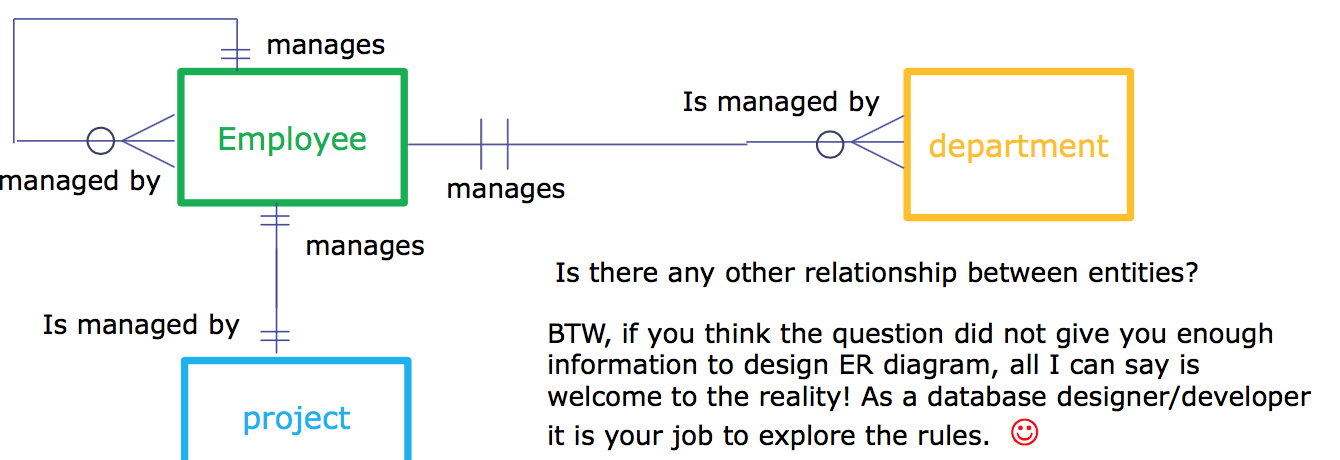
\includegraphics[scale=0.5]{lec3-2}

\subsection{Representing Multivalued Attribute}

It's generally not a good idea to have a multivalued attribute, as it can be represented as an attribute or an entity, and if it is represented by an entity, identifiers are needed for that entity. As an entity, it will result in a one to many relationship.

\subsection{Time -- Dependent Data}

Some data change their value over time and you may need to keep the history of this change. We would need to keep track of \textbf{Time stamps}, time values that is associated with a data value, often indicating when some event occurred that affected the data value.

\subsection{Enhanced ER diagram (EER)}

The ER model has been suitable for modelling most common business problems, but as business relationships get more complex, business data get more complex as well, so we would need a more complex tool to represent our model, such as an EER.\\
\\
An EER model is a model that has resulted from extending the original Entity Relationship model with new modelling constructs. The most important modelling construct incorporated in the EER model is the supertype/subtype relationships. The ideas of supertypes, subtypes and inheritance are the same parent-child concepts in object oriented software design. The only difference is that in object oriented programming, there is also the concept of behaviour, but in EER, the entities only inherit attributes.

\subsubsection{Attribute Inheritance}

Subtype entities inherit values of all attributes of the supertype, and an instance of a subtype is also an instance of a supertype.\\
\\
\underline{Examples:}\\
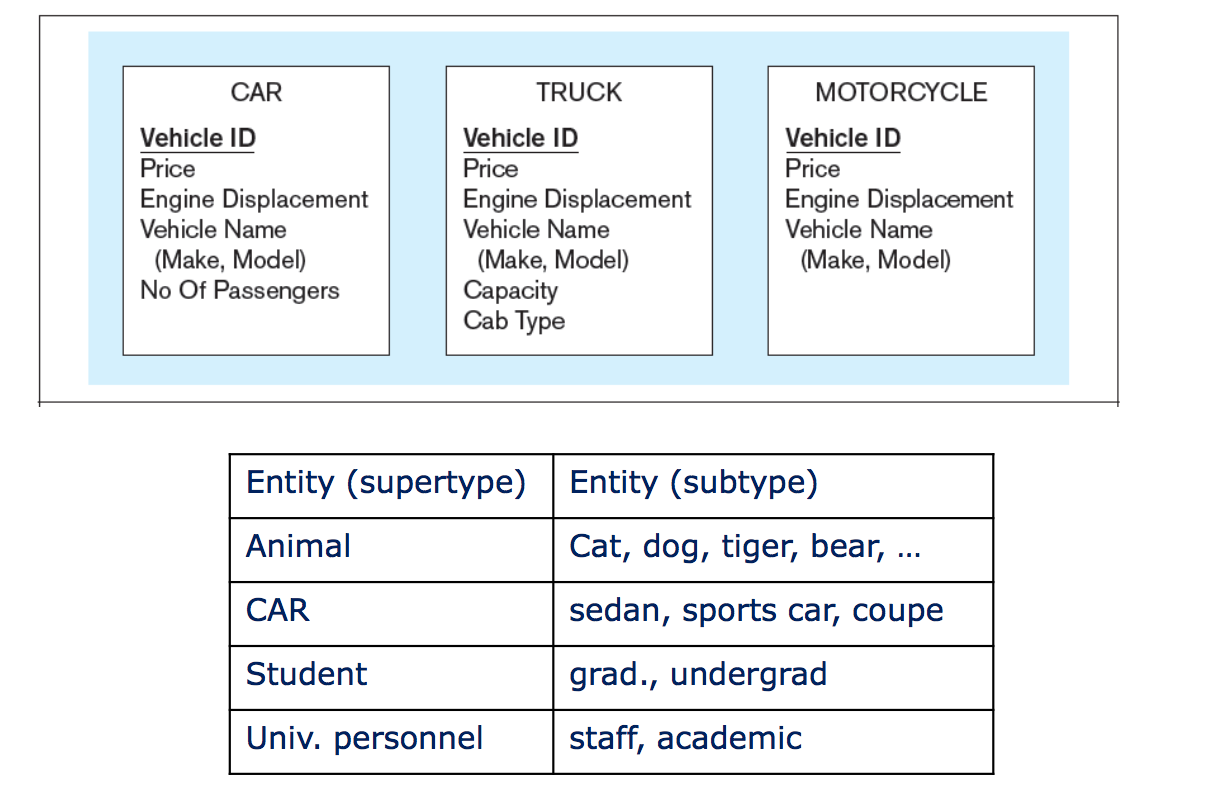
\includegraphics[scale=0.5]{lec3-3}\\
\\
and notation is as follows:\\
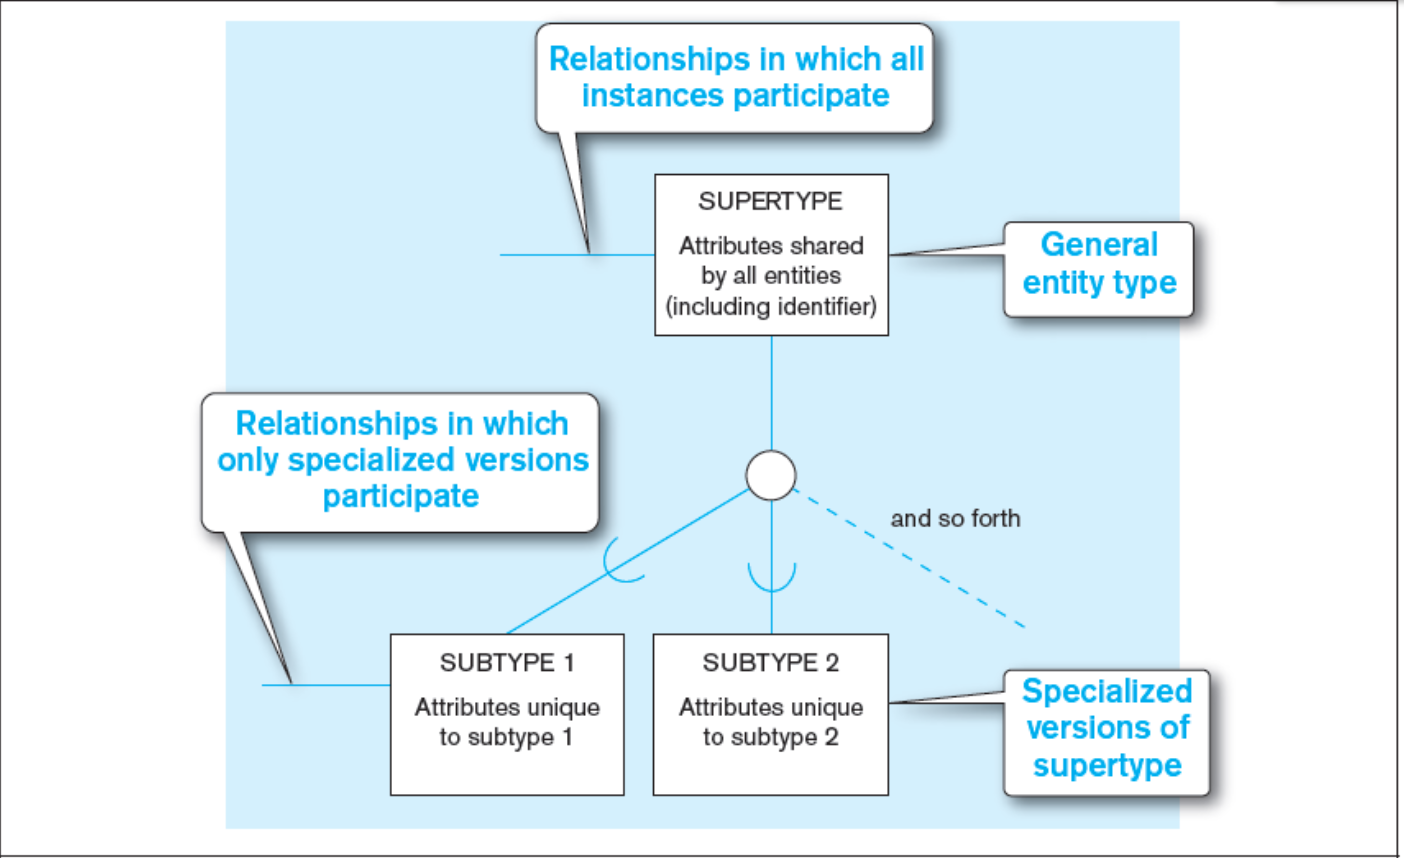
\includegraphics[scale=0.5]{lec3-4}

\subsection{Relationships}

Relationships at the supertype level indicate that all subtypes will participate in the relationship. The instances of a subtype may participate in a relationship unique to that subtype. In this situation, the relationship is shown at the subtype level.\\
\\
\underline{Example of Supertype/subtype relationships in a hospital:}\\
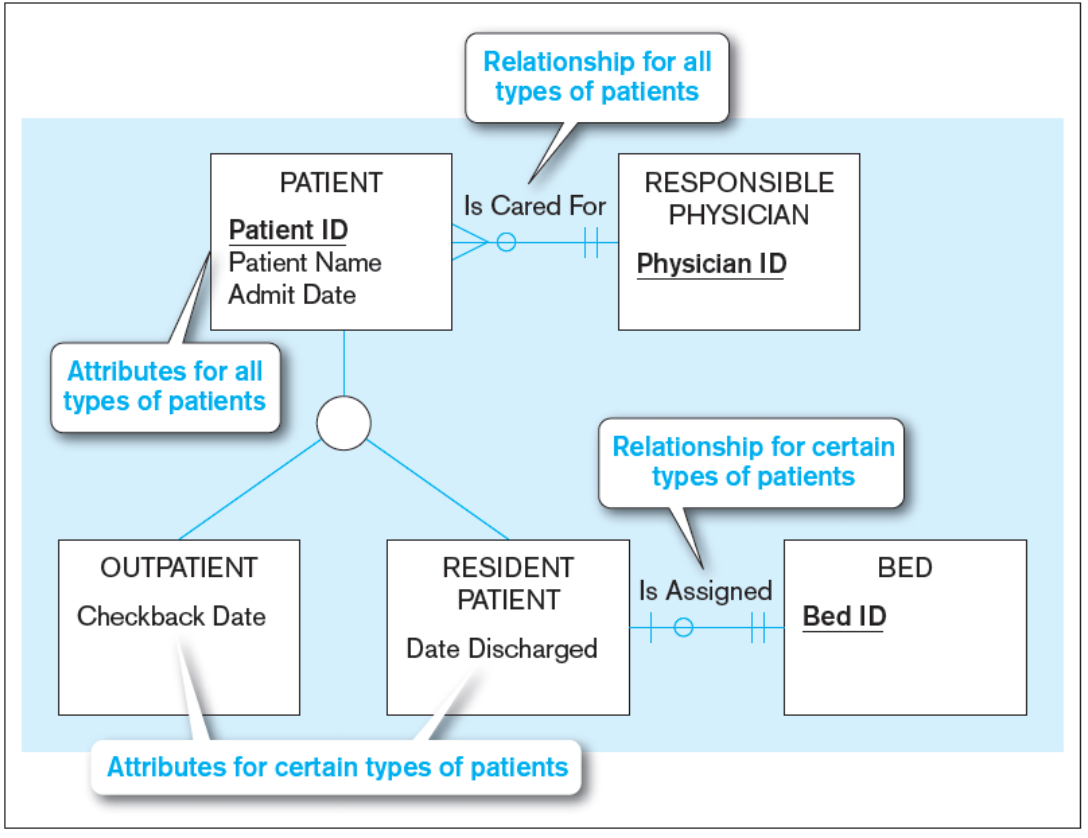
\includegraphics[scale=0.5]{lec3-5}

\subsection{Constraints in Relationship}

\textbf{Completeness Constraints} is whether an instance of a supertype must also be a member of at least one subtype. If yes, then this is a \textbf{total specialization rule} that is denoted by a double line, examples of total specialization include animal types being a specific species, paper publication types, etc. If no, then this is a \textbf{partial specialization rule}, and is denoted by a single line.\\
\\
\textbf{Disjointness Constraints} is whether an instance of a supertype may simultaneously be a member of two (or more) subtypes. If no (that an instance of the supertype can be only one of the subtypes at a time), then it is called the \textbf{Disjoint Rule} and is represented by a $d$, If yes (that an instance of the supertype could be more than one of the subtypes), then it is called the \textbf{Overlap Rule} and is represented by an $o$.\\
\\
\underline{Examples:}\\
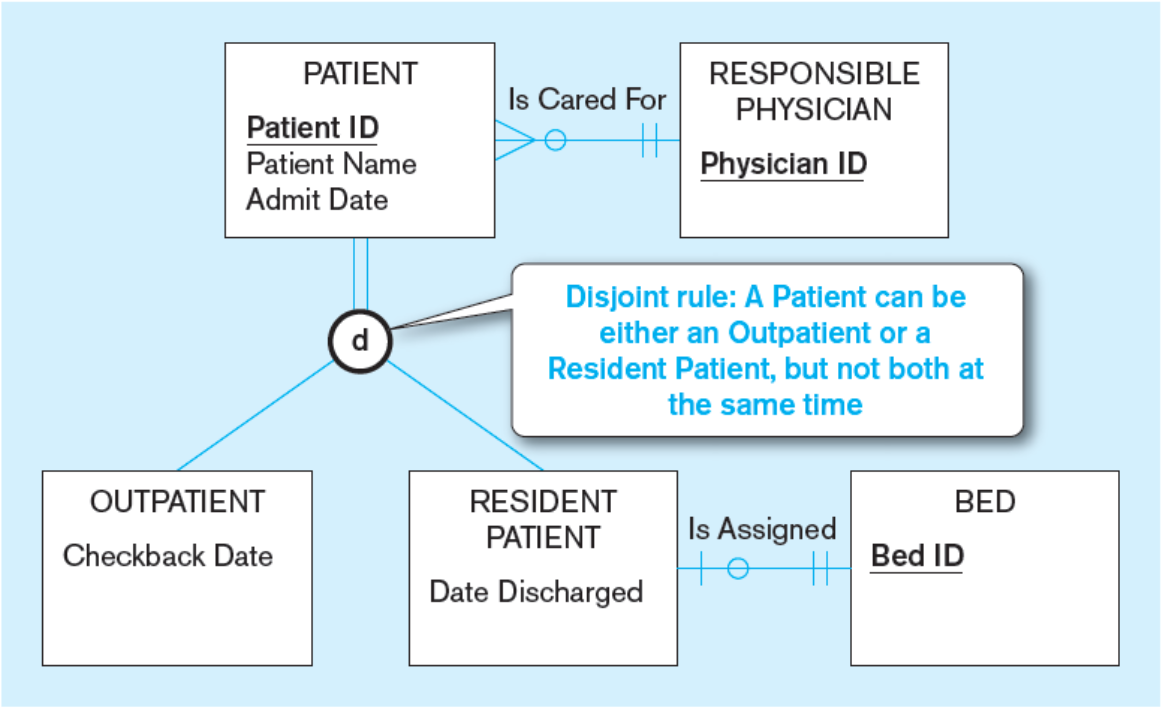
\includegraphics[scale=0.5]{lec3-6}\\
\\
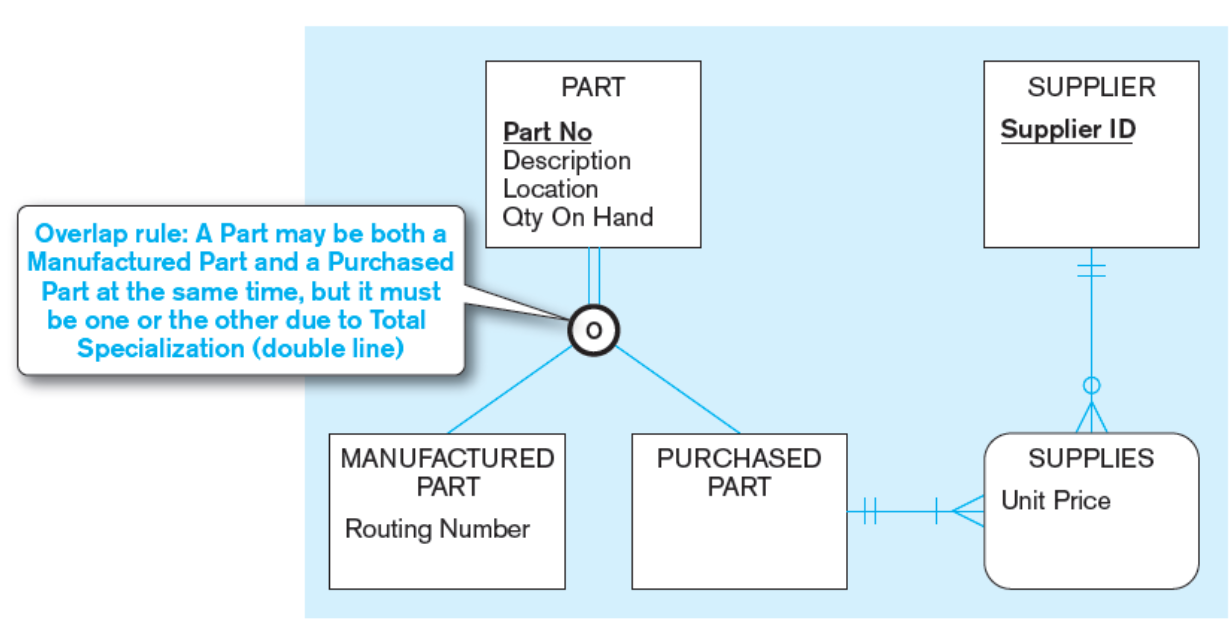
\includegraphics[scale=0.5]{lec3-7}

\subsection{Subtype Discriminator}

An attribute of the subtype whose values determine the target subtype. These subtypes are known as disjoint subtypes.\\
\\
\underline{Example of notation:}\\
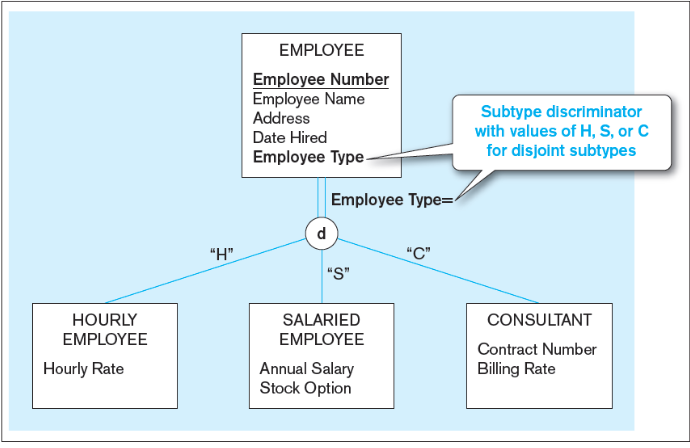
\includegraphics[scale=0.5]{lec3-8}\\

Overlapping also exists for subtype discriminators, it refers to a composite attribute whos subparts pertain to different subtypes. Each subpart contains a boolean value to indicate whether or not the instance belongs to the associated subtype.

\newpage

\section{Thursday, September 28, 2017}

\subsection{Database Design}

\textbf{Database design} is the process of converting EER Models into a relational data model. There are two steps for database design, Logical database design and Physical database design.

\subsection{Relational Data Model}

The relational data model has 3 components, one being the \textbf{Data structure}, such as tables (relations), rows, and columns. Another component being \textbf{Data manipulation}, such as using SQL to retrieve and modify data, and the last being \textbf{Data integrity}, which include mechanisms to implement business rules to maintain integrity of manipulated data.

\subsubsection{Relations}

A relation is a named 2-dimensional table of data, which consists of a set of named columns (attributes / fields) and an arbitrary number of rows (records). An example of short-hand notation of a relation would be (note that the underlined attribute is the identifier attribute): 
$$\text{EMPLOYEE1(\underline{EmpID}}, Name, DeptName, Salary)$$

\underline{Tables as Relations}\\
All relations are tables, but not all tables are relations. The requirements for a table to qualify as a relation are that the table must have a unique name, every attribute must be atomic (not multivalued nor composite), every row must be unique (so there cannot be two rows with the exact same values for all their fields), attributes in tables must have unique names, and the order of the columns and rows must be irrelevant.\\
\\
So in correspondence with the entity-relationship model, Entity Types become Relations, Entity Instances become Rows, and Columns become Attributes.

\begin{tcolorbox}
	\underline{Note:} the word \textbf{relation} in relational database is not the same as the word \textbf{relationship} in the E-R model.
\end{tcolorbox}

\subsubsection{Key Fields}

\paragraph{Primary Key} Primary keys are an attribute or combination of attributes that uniquely identifies each row in a relation. This (These) Primary key(s) must be the same as the identifier in the E-R model and must also be underlined for notation.

\paragraph{Composite Keys} Composite keys are a primary key that consists of more than one attribute.

\paragraph{Foreign Key} A foreign key is an identifier that enables a dependent relationship (on the many side of a relationship) to refer to its parent relation (on the side of the relationship). This foreign key is also no necessarily unique, is denoted by a dashed underlined, and represents a one to many relationship.

\underline{Example:}\\
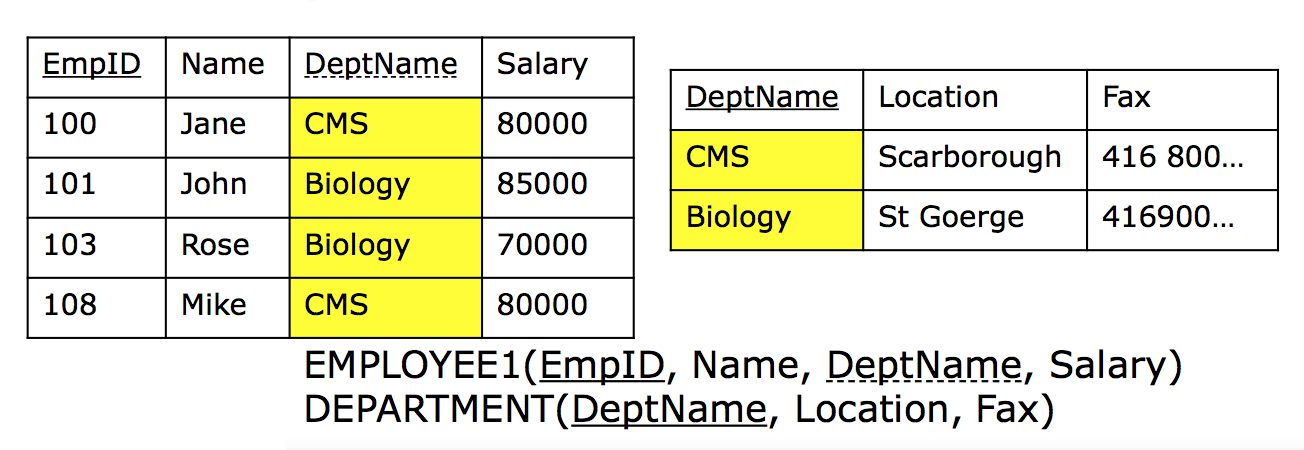
\includegraphics[scale=0.5]{lec4-1}

\subsubsection{Databases}

A Database is a collection of any number of relations, also known as a schema.\\
\\
\underline{Example:}\\
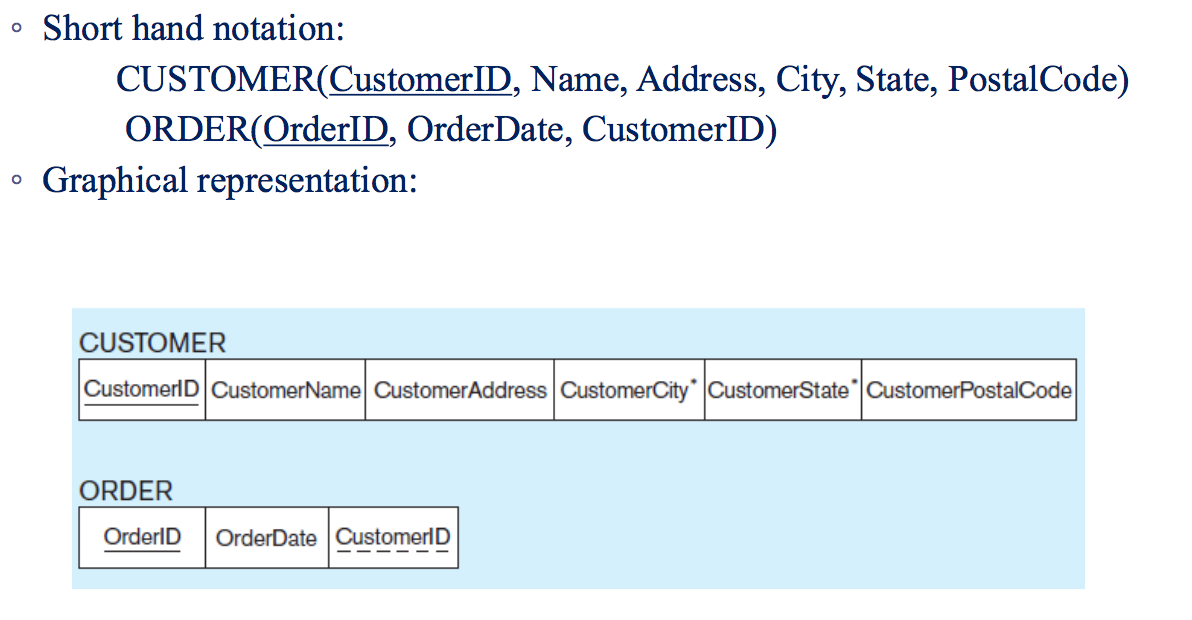
\includegraphics[scale=0.5]{lec4-2}

\subsubsection{Data Integrity}

Data Integrity is another component of a relational data model and more specifically, is the constraints or rules that assures the accuracy and integrity of data in the database. This component includes Domain Constraints, Entity Integrity, and Referential Integrity.

\paragraph{Domain Constraints} A domain constraint is a constraint that states that all values that appear in a column must original from the same domain, including the domain name \slash  data type, size and allowable values or range.
\\
\underline{Example:}\\
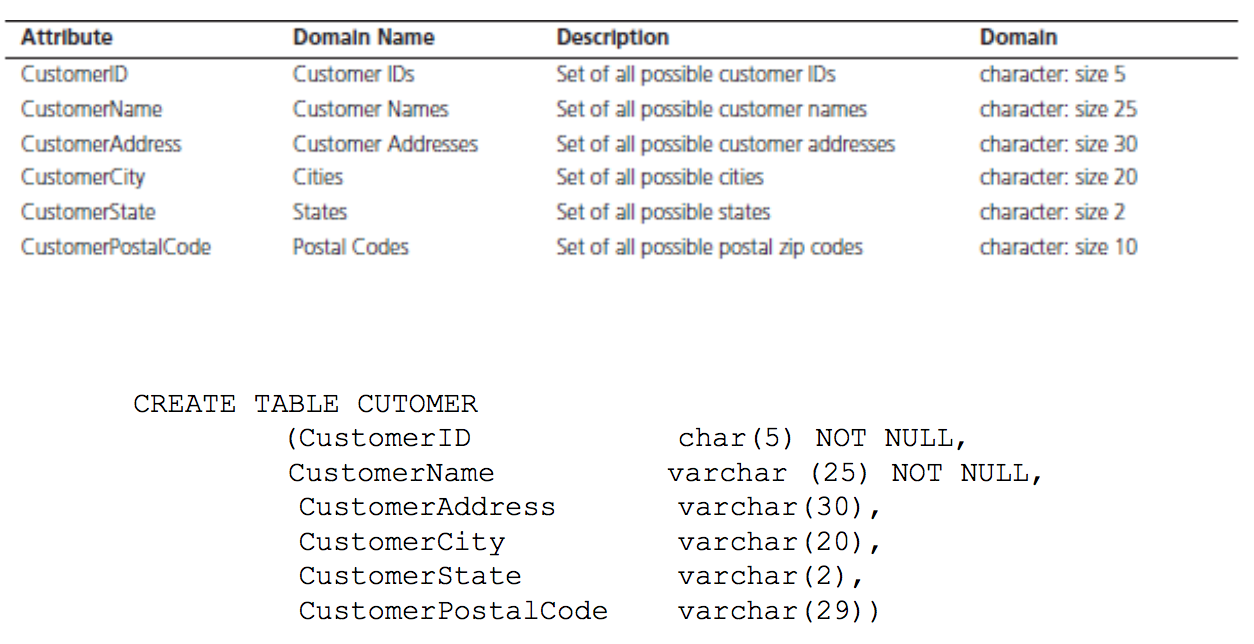
\includegraphics[scale=0.5]{lec4-3}

\paragraph{Entity Integrity} Entity Integrity means that each entity must have a primary key and that the primary key must not be null or nothing.

\paragraph{Referential Integrity} In a one to many relationship, any foreign key value (on the relation of the many side) must match a primary key value in the relation of the one side or the foreign key can be null
\\
\underline{Examples:}\\
\\
A patient may have many prescriptions assigned to them.
$$\text{Patient(\underline{PatientID}}, Name, Address)$$
$$\text{Patient(\underline{PerscriptionID}}, Name, \underline{PatientID})$$

\paragraph{Restrict Delete} When deleting an entity, entities that have other entities referring to them cannot be deleted. Only entities that are not referred to by other entities can be deleted.

\paragraph{Cascade Delete Rule} When deleting an entity, if an entity is referred to by other entities, those other entities will be deleted as well.

\paragraph{Set-to-Null Delete Rule} When deleting an entity, entities that referred to that entity before will now be referring to None.

\subsection{Transforming EER Diagrams into Relations}

Usually the job of transforming EER Diagrams into relations is usually done by the CASE tool, but it is still important to know the transformation process as the CASE tool cannot model complex data relations, such as Ternary and supertype \slash  subtype relations, there are sometimes legitimate alternatives where you will need to choose a particular solution, you must be able to perform quality check on the results obtained from the CASE tool.\\
\\
So for the transformation process, we must do the following:
\begin{enumerate}
	\item{Map Regular Entities}
	\item{Map Weak Entities}
	\item{Map Binary Relations}
	\item{Map Associative Relations}
	\item{Map Unary Relationships}
	\item{Map Ternary (n-ary) Relationships}
	\item{Map Supertype \slash  Subtype Relationships}
\end{enumerate}

\subsubsection{Map Regular Entities}

For Regular Entities, Entity types with simple attributes are made as a basic Relation, with a Relation Name, Relation Attributes and a Relation Primary Key. Entity types with composite attributes have each part of the composite attribute as a Relation attribute, and Entity types with multivalued attributes must create another relation for each multivalued attribute that refers back to the original Relation as the parent.

\subsubsection{Map Weak Entities}

Weak Entities correspond to a normal Relation but with a Surrogate Primary Key and a Foreign Key.

\subsubsection{Mapping Binary Relationships}

\paragraph{one to many} For one to many binary relationships between entities, each element in the many relationship must also have a foreign key corresponding to the ID of the on element.

\paragraph{many to many} For many to many binary relationships between entities, each matching between the two many entity types must have a certificate with two foreign keys in which one refers to one entity type and the other refers to the other entity type. This certificate composite primary key will be the foreign keys.

\paragraph{one to one} For one to one relationships, we let the mandatory relation have a foreign key of the other relation. For mandatory one to one relationships, we can have both relations have foreign keys to the other relation.

\newpage

\section{Thursday, October 5, 2017}

\subsection{Mapping EER into Relations}

\subsubsection{Mapping Associate Entities}

If the identifier is not assigned, associate entities become a relation with foreign keys to its respective parent relations as well as a composite primary key formed from the two foreign keys previously mentioned.\\
\\
If the identifier is assigned, do as before, but the Primary key differs from the foreign keys.

\subsubsection{Mapping Unary Relationships}

For one to one or one to many relationships, the entity is turned into a relation that has a recursive foreign key (the foreign key refers to the primary key of the relation of the same type).\\
\\
For many to many relationships, attributes that come with these relationships are put in a separate component relation with those attributes as well as the two foreign keys for the two sides of the relationship as its composite keys.

\subsubsection{Mapping Ternary (and n-ary) Relationships}

When mapping ternary (and n-ary) relationships, it is simply adding a foreign key in the relation that corresponds to the entity with an optional existence.\\
\\
\underline{Example:}\\
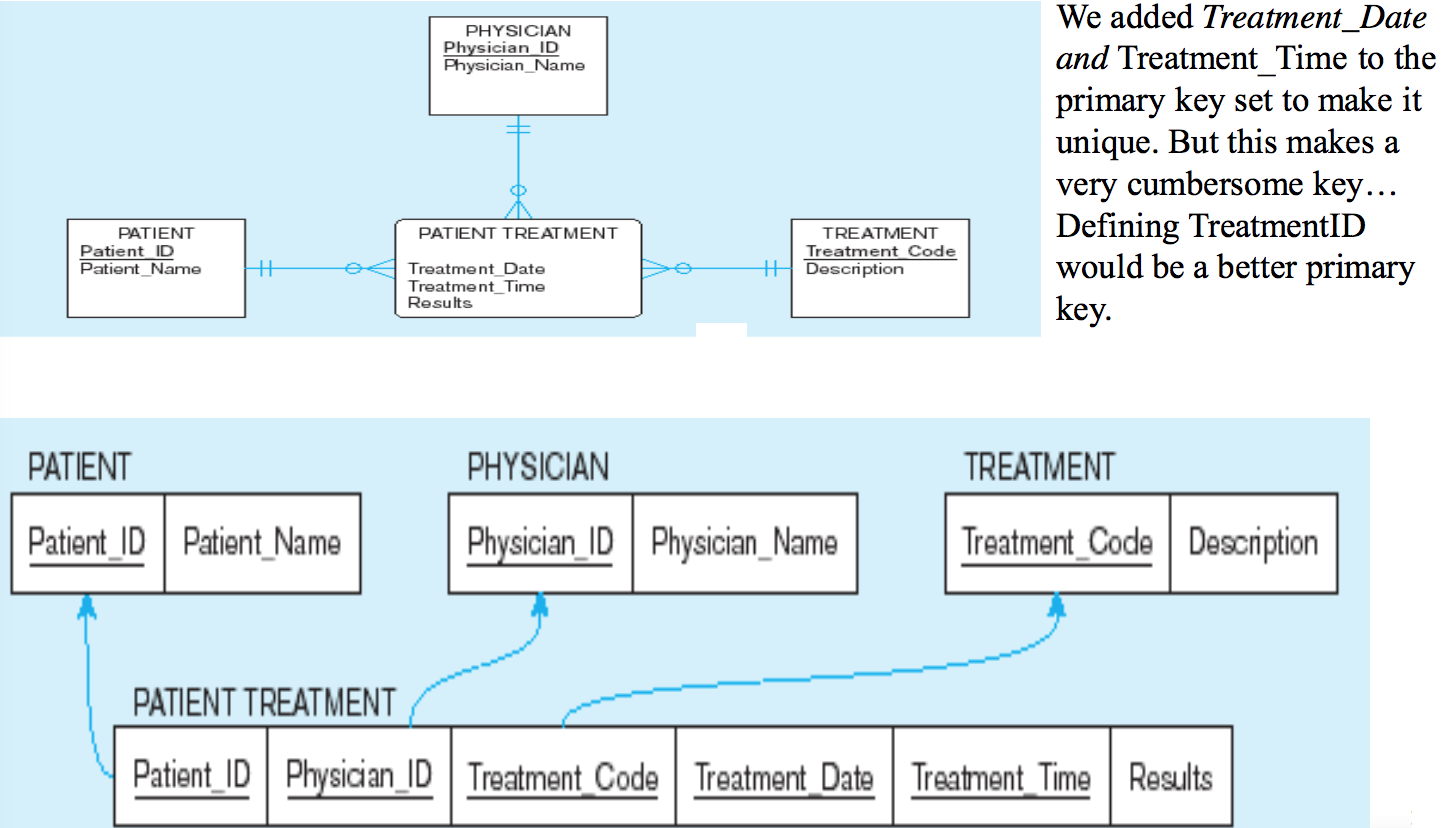
\includegraphics[scale=0.5]{lec5-1}

\subsubsection{Mapping Supertype \slash  Subtype Relationship}

To map these types of relationships, we implement one to one relationships between the subtype and the supertype. So the relations of the subtype must include supertype attributes, a subtype primary key, and a subtype discriminator. The supertype must essentially be a primary table.\\
\\
\underline{Example:}\\
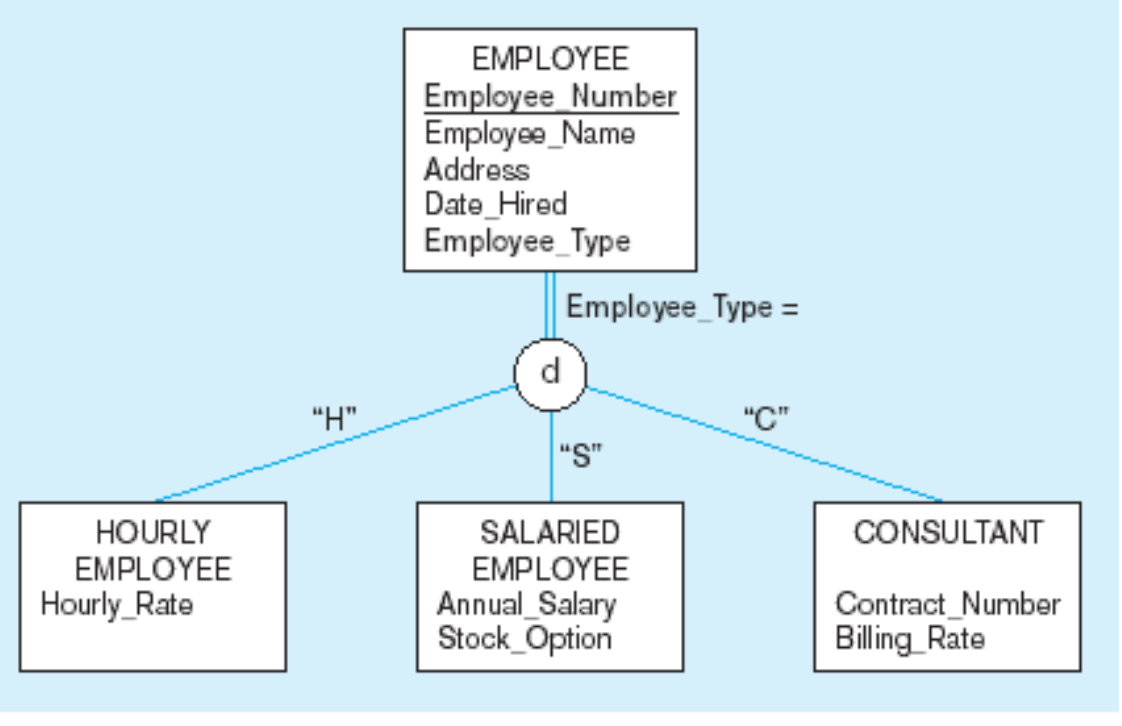
\includegraphics[scale=0.7]{lec5-2}\\
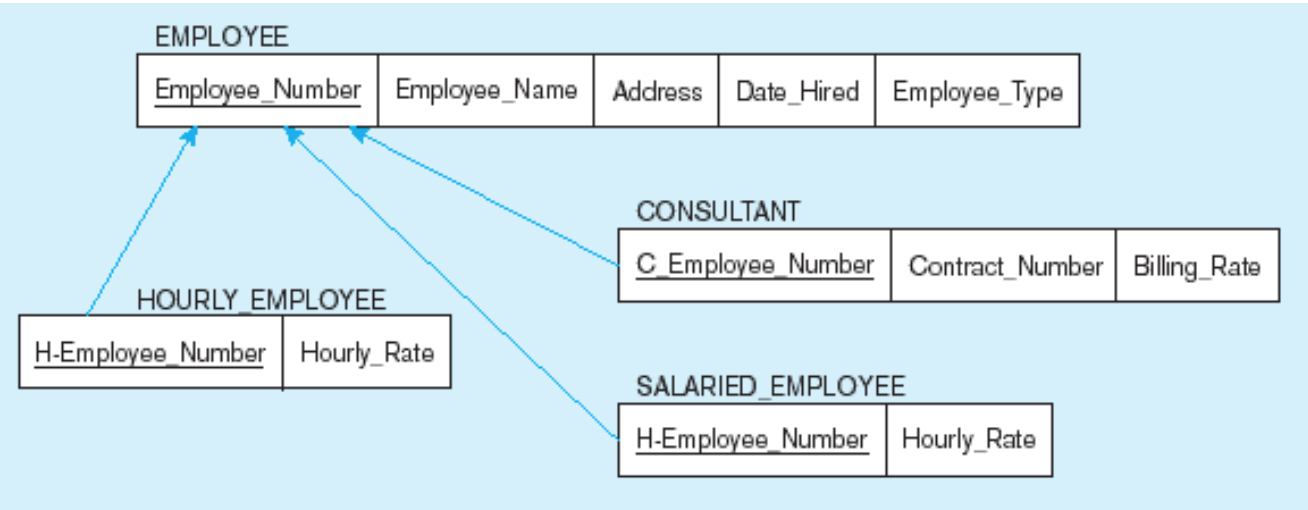
\includegraphics[scale=0.6]{lec5-3}

If the constraint in supertype \slash  subtype followed the overlap rule, we can let the discriminator take on multiple values (for each subtype to have attributes for each discriminator type taking on a boolean stating if that relation is that type of discriminator or not). This can also accommodate the completeness constraint, if it was partial rather than total.

\subsection{Normalization}

There is no guarantee that transforming EER diagrams to relations will remove all the anomalies. \textbf{Normalization} is the process of decomposing relations with anomalies to produce smaller well-structured relations.
\subsubsection{Properties of Well-Structured Relations}
\begin{itemize}
	\item{\textbf{No Data Redundancy}}
	\item{\textbf{No Insertion Anomalies}, which refers to adding new rows to a Table, adding new rows should not force the user to insert some irrelevant data}
	\item{\textbf{No Deletion Anomalies}, which refers to deleting rows and that deleting rows should not cause a loss of data that could be needed for other future rows}
	\item{\textbf{No Modification Anomaly}, which refers to changing data in a row should not force changes to other rows because of duplications}
\end{itemize}

\subsubsection{Steps in Normalization}

\paragraph{First Normal Form (1NF)} The First Normal Form is not allowed to have multivalued attributes, and every attribute value must be atomic. All relations are in the 1st Normal Form, but this does not prevent anomalies from existing.

\paragraph{Functional Dependency} Functional Dependency is when the value of one attribute (the \textbf{determinant}) determines the value of another attribute. Examples include: \textit{CustomerID} being a determinant because it determines the value of the \textit{CustomerName}. Functional Dependency is represented by an arrow, i.e. $A \rightarrow B$

\paragraph{Candidate Keys} A candidate key is a unique identifier, could be an attribute or a combination of attributes that uniquely identifies a row in a relation. One of the candidate keys will become the primary key. Candidate keys are also non-redundant, no attribute in the key can be deleted without destroying the property of unique identification. Note that each non-key field is functionally dependent on every candidate key.\\
\\
Examples include:\\
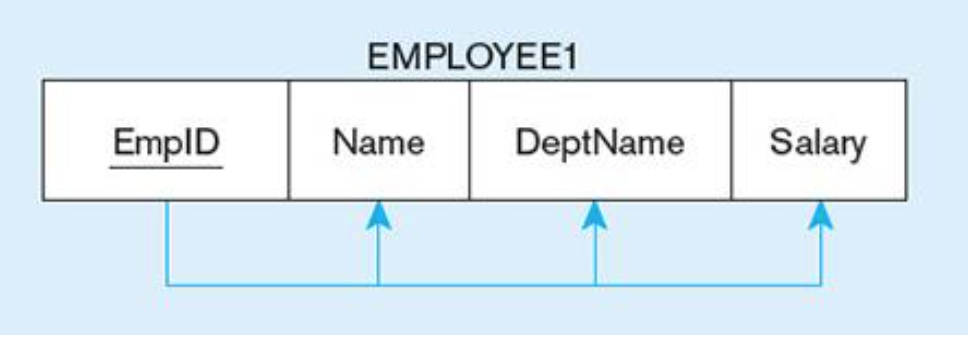
\includegraphics[scale=0.8]{lec5-4}\\
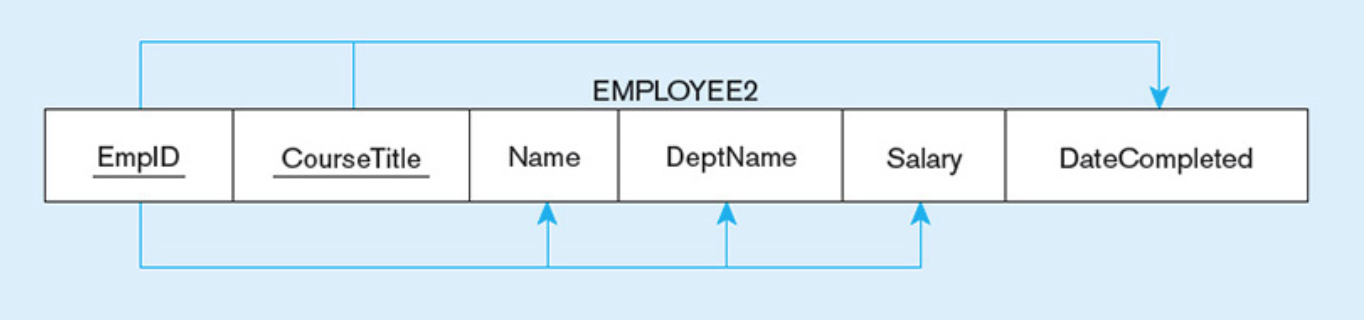
\includegraphics[scale=0.5]{lec5-5}

\end{document}









































